\documentclass[a4paper,11pt,oneside,fleqn]{report}

\usepackage{amsmath,amsthm,amssymb}

\usepackage[UKenglish]{babel}

\usepackage{xcolor}
\usepackage{graphicx}

\usepackage{booktabs}
\usepackage{caption}

\newcommand{\Ncoils}{N_{\textup{coils}}}
\newcommand{\Nturns}{N_{\textup{turns}}}
\newcommand{\Nlayers}{N_{\textup{layers}}}


\title{3F --- Framework for \textsc{Femm}}
\author{}

\begin{document}
\maketitle
\tableofcontents

\chapter{Geometry}

\section{Slots}
\makebox[1\textwidth][c]{
\begin{tabular}{ccccccc}
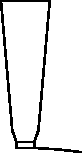
\includegraphics{../examples/slots/squared_slot} &
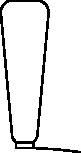
\includegraphics{../examples/slots/rounded_slot} &
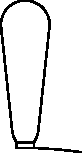
\includegraphics{../examples/slots/round_slot} &
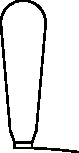
\includegraphics{../examples/slots/semiround_slot} &
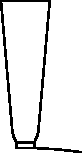
\includegraphics{../examples/slots/roundsemi_slot} &
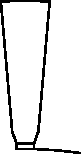
\includegraphics{../examples/slots/semiarc_slot} &
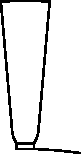
\includegraphics{../examples/slots/roundarc_slot} \\
%
\texttt{squared} &
\texttt{rounded} &
\texttt{round} &
\texttt{semiround} &
\texttt{roundsemi} &
\texttt{semiarc} & 
\texttt{roundarc}
\end{tabular}}
\vspace{1cm}


% Stators
\newpage
\section{Stators}
\begin{tabular}{c}
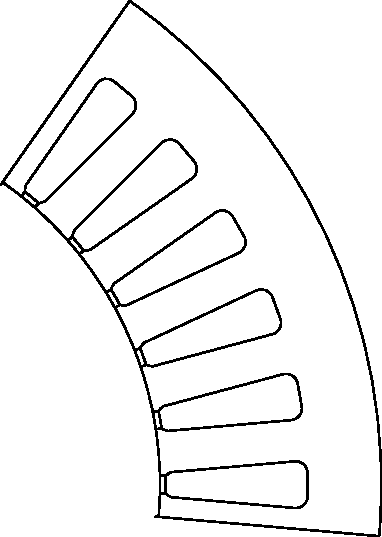
\includegraphics[scale=0.75]{../examples/stators/1pole} 
\\
$ 1 $ \texttt{pole}
\end{tabular}
\vspace{5mm}

\begin{tabular}{c}
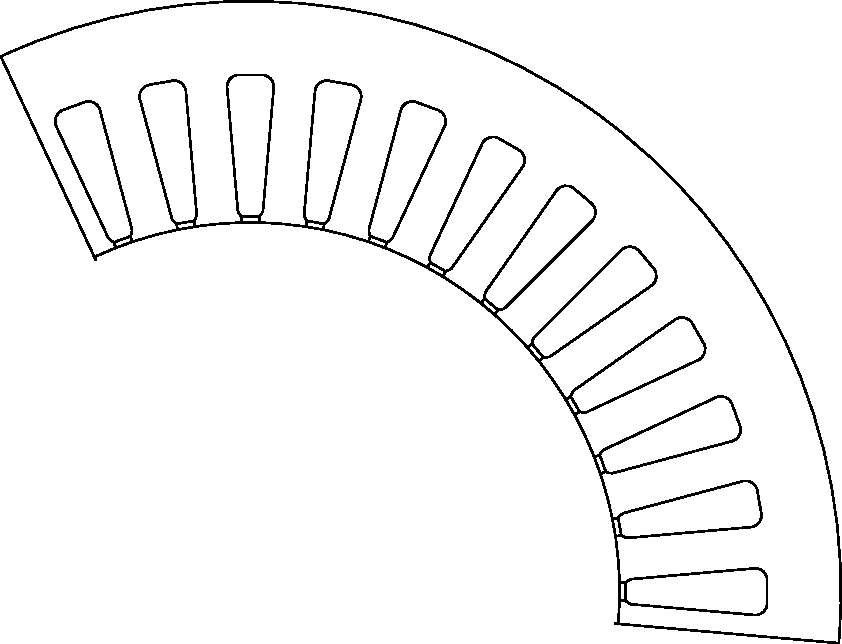
\includegraphics[scale=0.75]{../examples/stators/2pole} 
\\
$ 2 $ \texttt{poles}
\end{tabular}
\vspace{5mm}

\begin{tabular}{c}
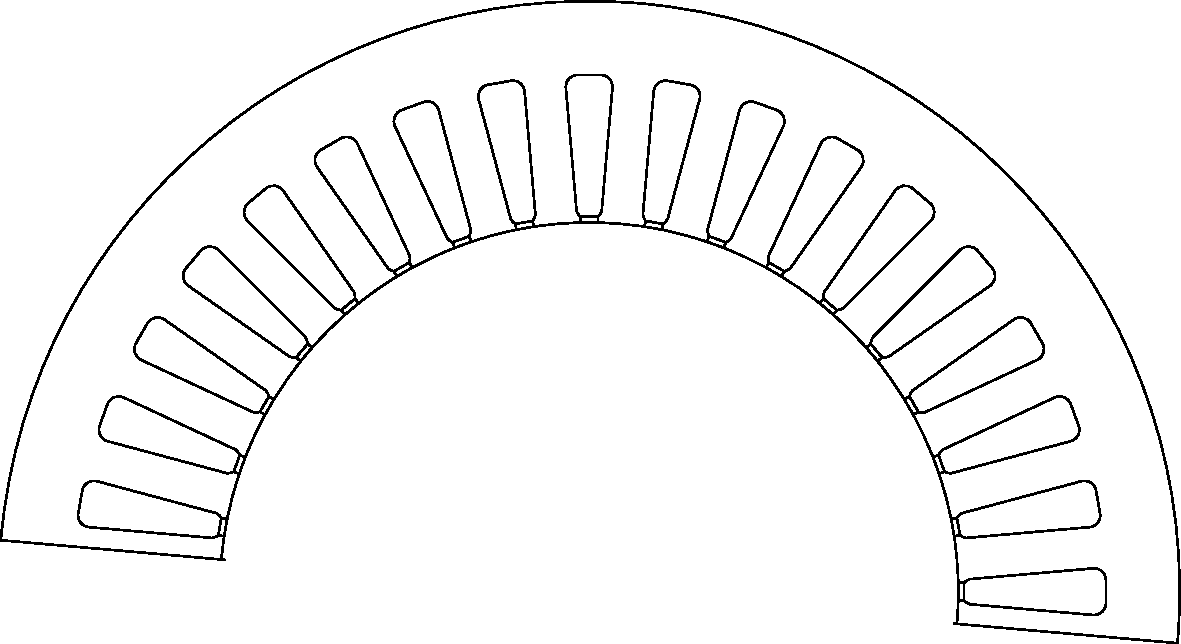
\includegraphics[scale=0.75]{../examples/stators/ppole} 
\\
$ p $ \texttt{poles}
\end{tabular}
\vspace{5mm}

\begin{tabular}{c}
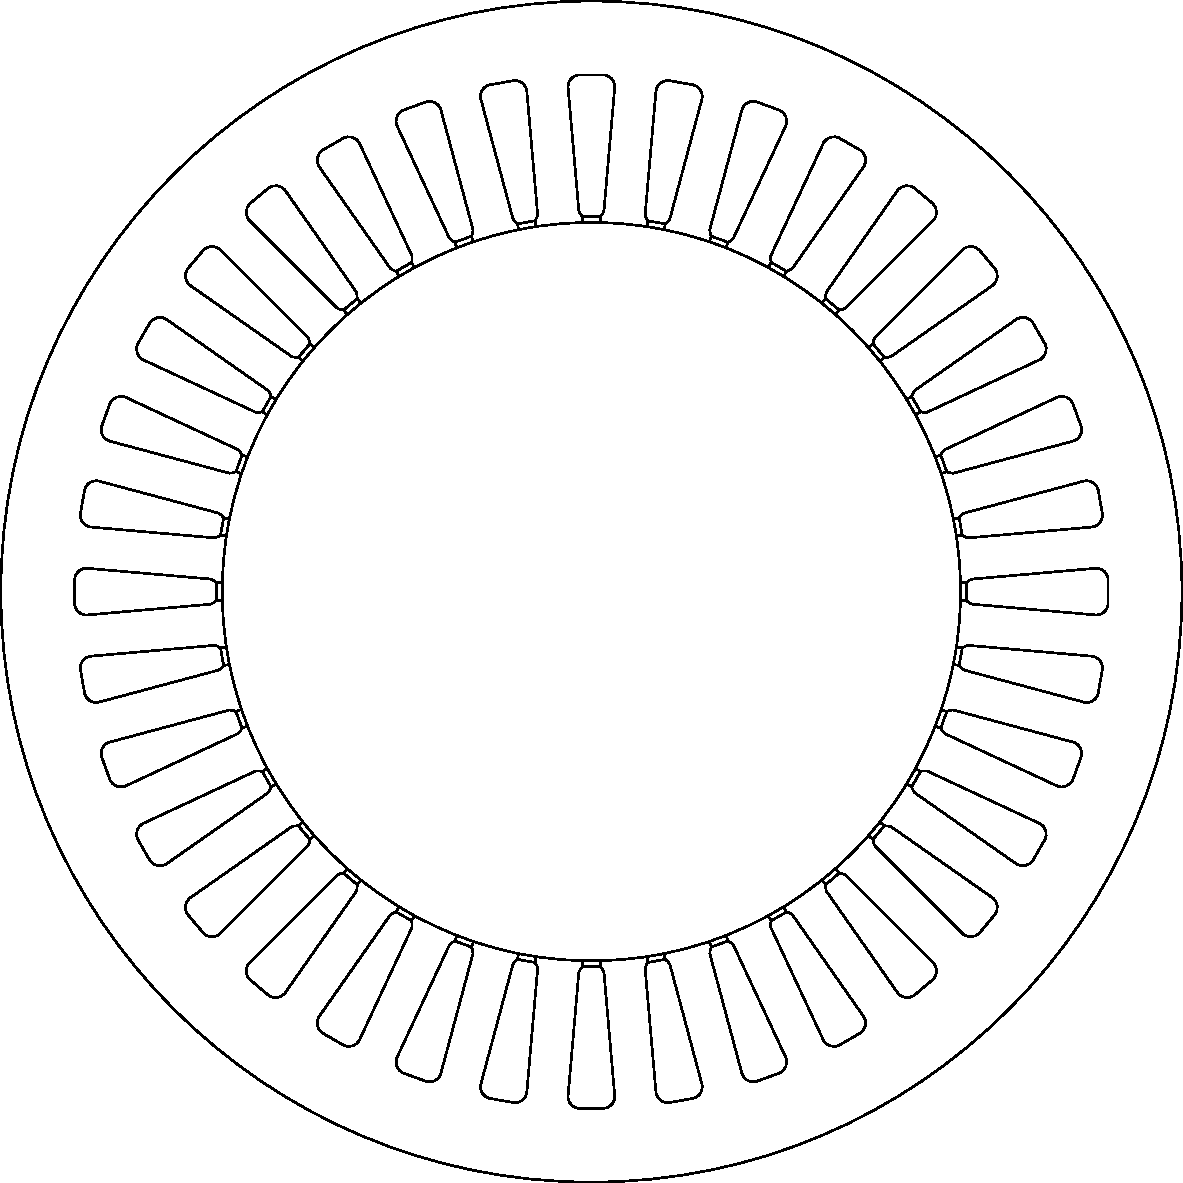
\includegraphics[scale=0.75]{../examples/stators/2ppole}
 
\\
$ 2p $ \texttt{poles}
\end{tabular}



% Magnets
\newpage
\section{SPM Magnets}

\begin{tabular}{c}
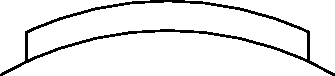
\includegraphics[scale=1]{../examples/magnets/parallel_rect}
\\
\texttt{parallel + rect}
\end{tabular}
\vspace{5mm}

\noindent
\begin{tabular}{c}
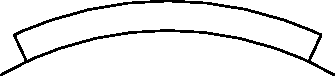
\includegraphics[scale=1]{../examples/magnets/parallel_trapz}
\\
\texttt{parallel + trapz}
\end{tabular}
\vspace{5mm}

\noindent
\begin{tabular}{c}
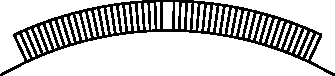
\includegraphics[scale=1]{../examples/magnets/radial_trapz}
\\
\texttt{radial (+ trapz)}
\end{tabular}




% Rotors
\newpage
\section{SPM Rotors}
\begin{tabular}{c}
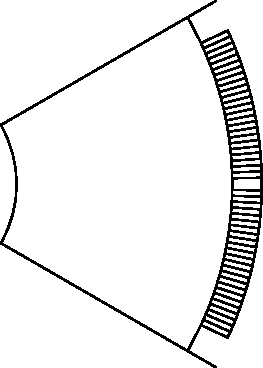
\includegraphics[scale=0.75]{../examples/rotors/1pole} 
\\
$ 1 $ \texttt{pole}
\end{tabular}
\vspace{5mm}

\begin{tabular}{c}
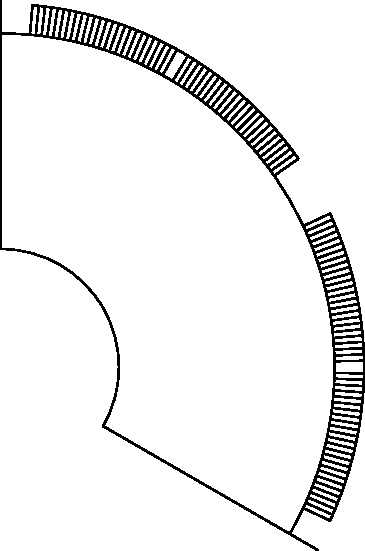
\includegraphics[scale=0.75]{../examples/rotors/2pole} 
\\
$ 2 $ \texttt{poles}
\end{tabular}
\vspace{5mm}

\begin{tabular}{c}
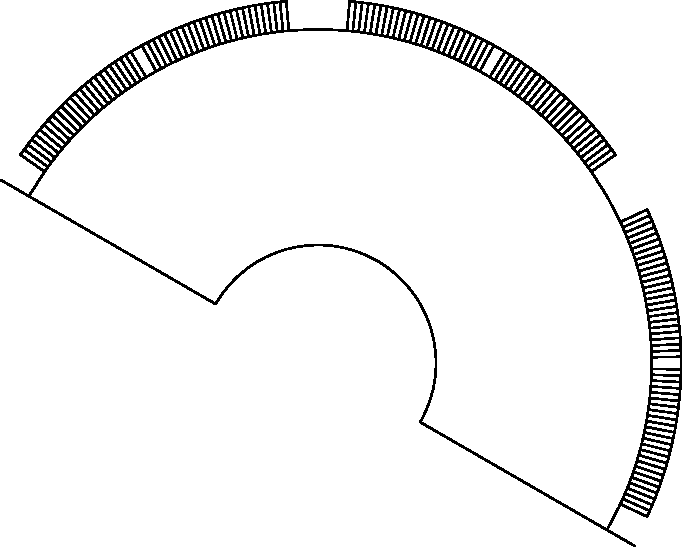
\includegraphics[scale=0.75]{../examples/rotors/ppole} 
\\
$ p $ \texttt{poles}
\end{tabular}
\vspace{5mm}

\begin{tabular}{c}
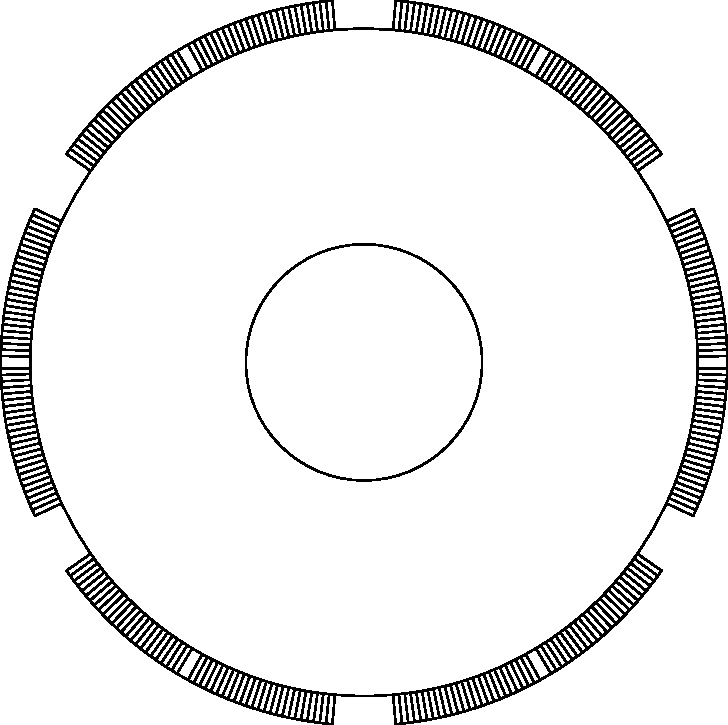
\includegraphics[scale=0.75]{../examples/rotors/2ppole} 
\\
$ 2p $ \texttt{poles}
\end{tabular}






\chapter{Winding}
We will characterise a winding through

\begin{table}[h]
\centering
\begin{tabular}{lll}
\toprule
Name         & Math symbol    & Code symbol 
\\\midrule
%
N. of phases & $ m $          & \texttt{m} 
\\
N. of coils  & $ \Ncoils $ & 
\texttt{coils} \\
N. of turns per coil & $ \Nturns $ & 
\texttt{turns} \\
N. of layers & $ \Nlayers $ & \texttt{layers} \\
\bottomrule
\end{tabular}
\end{table}

Typically, given a lamination stack with $ Q $ slots
\begin{equation*}
\Ncoils = \frac{Q}{2}\,\Nlayers
\end{equation*}
so if the number of layers is one, the number of coils is 
half the number of slots, given the fact that a coil side 
occupies a full slot.



\end{document}